\chapter{strongTNC}

\section{Requirements}
\section{Zweck}


\section{Nichtfunktionale Anforderungen}
Da es sich um eine Erweiterung eines bestehenden Systemes handelt, sollen die
Anforderungen die für die Basis definiert wurden auch für die Erweiterung
gelten. Als neue Requirements wurden folgende Punkte definiert:
\begin{itemize}
	\item Die Software soll nicht über ein Paketmanager installierbar sein, die
	Möglichkeit immer aktuelle Software Versionen einzusetzen ist wichtiger
	\item Der ISO Standard 19770-2:2014 soll eingehalten werden.
\end{itemize}

\subsection{Use Cases}

Nachfolgend werden die identifizierten Use Cases beschrieben. Als
\enquote{System under Decision} wird die strongTNC Django Webapp als Ganzes
betrachtet.

\subsubsection{UC01: CMDB, Softwareinventar eines Gerätes}
\begin{usecase}
\hline
\textbf{Akteur} & strongTNC Benutzer \\
\hline
\textbf{Story} &
Der Akteur will feststellen, welche Software in welcher Version zu einem
bestimmten Zeitpunkt auf einem Gerät installiert war.\\
\hline
\textbf{Standard Szenario} &
Der Akteur betrachtet das SWID Tag Inventar des gewünschten Gerätes und kann
dort zu jedem Mess-Zeitpunkt die installierte Software abrufen. \\
\hline
\textbf{Alternatives Szenario} &
% TODO dies ist eine alternative story, kein alternatives szenario.
Der Akteur möchte wissen auf welchen Geräten eine bestimmte Software Version
installiert ist oder war (beispielsweise weil in dieser Version eine kritische
Sicherheitslücke enthalten ist). Der Akteur wählt dazu den gewünschten SWID Tag
in der SWID Liste und die Geräte welche die Software installiert hatten werden
aufgelistet.\\
\hline
\end{usecase}

\subsubsection{UC02: Detaillierte SWID-Tag File Information}
\begin{usecase}
\hline
\textbf{Akteur} & strongTNC Benutzer \\
\hline
\textbf{Story} &
Der Akteur will feststellen welche Dateien zu einem bestimmten Softwarepaket gehören. \\
\hline
\textbf{Standard Szenario} &
Der Akteur findet den SWID Tag der zum gesuchten Softwarepaket gehört in der
SWID Tag Ansicht. Die Dateien die mit dem SWID Tag gemessen wurden sind
aufgelistet. \\
\hline
\textbf{Alternatives Szenario} & 
Der Akteur findet das Softwarepaket in der Paketübersicht. Dort kann auf einen
verknüpfen SWID Tag zugegriffen werden. So gelangt der Akteur auf die SWID Tag
Ansicht und findet dort die Liste der gemessenen Dateien. \\
\hline
\end{usecase}

\subsubsection{UC03: Entities auflisten}
\begin{usecase}
\hline
\textbf{Akteur} & strongTNC Benutzer \\
\hline
\textbf{Story} &
Der Akteur will alle im System erfassten Entites auflisten und herausfinden
welche SWID Tags zu der jeweiligen Entity gehören. \\
\hline
\textbf{Standard Szenario} &
Der Akteur kann sich in der Entity Ansicht alle erfassten Entities auflisten lassen. Wenn eine Entity angewählt wird, werden alle SWID Tags, die der Entity zugeordnet sind, aufgelistet. \\
\hline
\phantom{\textbf{Alternatives Szenario}} & 
\end{usecase}

\subsubsection{UC04: Verfügbare SWID-Tags auflisten}
\begin{usecase}
\hline
\textbf{Akteur} & strongTNC Benutzer \\
\hline
\textbf{Story} &
Der Akteur will alle im System erfassten SWID Tags auflisten. Dabei ist er an folgenden Informationen eines Tags interessiert:
\begin{itemize}
\item Software-ID
\item Unique ID
\item Tag Creator Entity
\item RAW XML String
\item Welche Files sind in diesem SWID Tag enthalten.
\item Gibt es ein bestehendes Paket dessen Name dem des SWID Tags entspricht.
\item Welche Devices haben diesen SWID Tag installiert gemeldet (TODO siehe Use Case UC01)
\end{itemize}\\
\hline
\textbf{Standard Szenario} &
Der Akteur kann sich in der SWID Tag Ansicht alle erfassten SWID Tags auflisten lassen. Wenn ein SWID Tag angewählt wird, sind alle gewünschten Details aufgelistet. \\
\hline
\phantom{\textbf{Alternatives Szenario}} &
\end{usecase}

\subsubsection{UC05: Erfassen eines neuen SWID-Tags}
\begin{usecase}
\hline
\textbf{Akteur} & strongSwan TNC Server oder Administrator\\
\hline
\textbf{Story} &
Der Akteur will einen neuen SWID Tag im System erfassen. Der Akteur liefert ein XML Dokument gemäss SWID Spezifikation (TODO Reference) an das System. Das System nimmt das XML Dokument entgegen und speichert die notwendigen Informationen ab.\\
\hline
\textbf{Standard Szenario} &
Der Akteur liefert ein XML Dokument an das System und erhält eine Erfolgsmeldung die bestätigt, dass der Tag gespeichert wurde.\\
\hline
\textbf{Alternatives Szenario 1} & 
Eine Entity welche im gelieferte XMl enthalten ist exisitiert bereits im System (identifiziert durch die regid) besitzt aber einen anderen Namen. Der Name der bestehenden Entity wird entsprechend aktualisiert.\\
\hline
\textbf{Alternatives Szenario 2} & 
Der Tag welcher erfasst werden sollte existiert bereits im System, identifiziert durch die software-id (TODO Referenz).
\begin{description}
\item[2a] Die Erfassung eines neuen SWID Tags erfolgt programmatisch über die TNC Server Komponente. Ein Tag mit derselben Unique ID existiert bereits und wird nicht ersetzt.
\item[2b] Die Erfassung eines neuen SWID Tags erfolgt manuell durch den Administrator. Ein Tag mit derselben Unique ID existiert bereits und wird mit den neuen Daten ersetzt.
\end{description}
\\
\hline
\textbf{Alternatives Szenario 3} & 
Es wurde ein invalides XML Dokument ans System geliefert. Das System informiert den Benutzer über den Fehler und erstellt keinen neuen Tag.\\
\hline
\textbf{Häufigkeit des Auftretens} &
Bei Systemeinführung wird diese Operation häufig auftreten. Idealerweise sieht das Deployment vor, dass für jeden Produktetyp ein Referenzgerät vorhanden ist, mit welchem initial alle Tags generiert und erfasst werden und danach in regelmässigen Abständen aktualisiert werden. Dadurch ist die Anzahl der nötigen Erfassungs-Operationen durch User Endgeräte klein zu halten.\\
\hline
\end{usecase}

\subsubsection{UC05: Durchführen einer SWID Messung für ein Gerät}
\begin{usecase}
\hline
\textbf{Akteur} & strongSwan TNC Server \\
\hline
\textbf{Story} &
Der Akteur will alle auf einem Device vorhandenen SWID Tags mit einer Session verknüpfen\\
\hline
\textbf{Standard Szenario} &
Der Akteur sendet eine Liste der software-ids an das System die er mit der aktuellen Session verknüpfen möchte. Der Server assoziert die entsprechenden Tags mit der Session und bestätigt den erfolgreichen Vorgang.\\
\hline
\textbf{Alternatives Szenario} & 
Es existieren nicht für alle gelieferten software-id's Tags im System. Das System assoziiert keine Tags mit der aktuellen Session und gibt eine Liste derjenigen software-id's zurück für welche keine Tags vorhanden sind. Der Akteur erfasst darauf hin alle Fehlenden Tags im System. Sobald alle Tags im System erfasst sind tritt das Standard Szenario ein.
\end{usecase}

\subsubsection{Auflisten aller Tags zu einem File}
\begin{usecase}
\hline
\textbf{Akteur} & strongTNC Benutzer \\
\hline
\textbf{Story} &
Der Akteur will alle im System erfassten Entites auflisten und herausfinden
welche SWID Tags zu der jeweiligen Entity gehören. \\
\hline
\textbf{Standard Szenario} &
Der Akteur kann sich in der Entity Ansicht alle erfassten Entities auflisten lassen. Wenn eine Entity angewählt wird, sind alle SWID Tags die der Entity zugeordnet sind Aufgelistet. \\
\hline
\phantom{\textbf{Alternatives Szenario}} & 
\end{usecase}

Der Benutzer kann auflisten, welche Tags ein bestimmtes File enthalten.



\section{SWID Erweiterung}
\section{Datenmodellierung}
Die Erweiterung des bestehenden Datenmodells ist in Abbilung (TODO Referenz) zu sehen. Die hinzugefügten Tabellen sind im grünen Teil hervorgehoben. Bei den Tabellen mit grauen Rahmen handelt es sich um Zwischentabellen, welche eine N zu N Beziehung auflösen. Beim modellieren der zusätzlichen Tabellen wurde darauf geachtet, dass keine bestehenden Tabellen geändert werden müssen. Die Beziehungen werden daher alle von extern, seitens der Erweiterung, hergestellt.
\begin{description}
\item [swid\_entities] Ein SWID Tag kann mehrere Entities enthalten. Entities haben in einem Tag eine Rollen oder eine beliebige Kombination aus (Tag creator, Publisher oder Licensor). Pro SWID Tag darf es aber nur einen Tag creator geben. Dieser Constraint wird aber erst in den Models vom ORM (TODO Glossar)

\end{description}
\begin{figure}
\centering
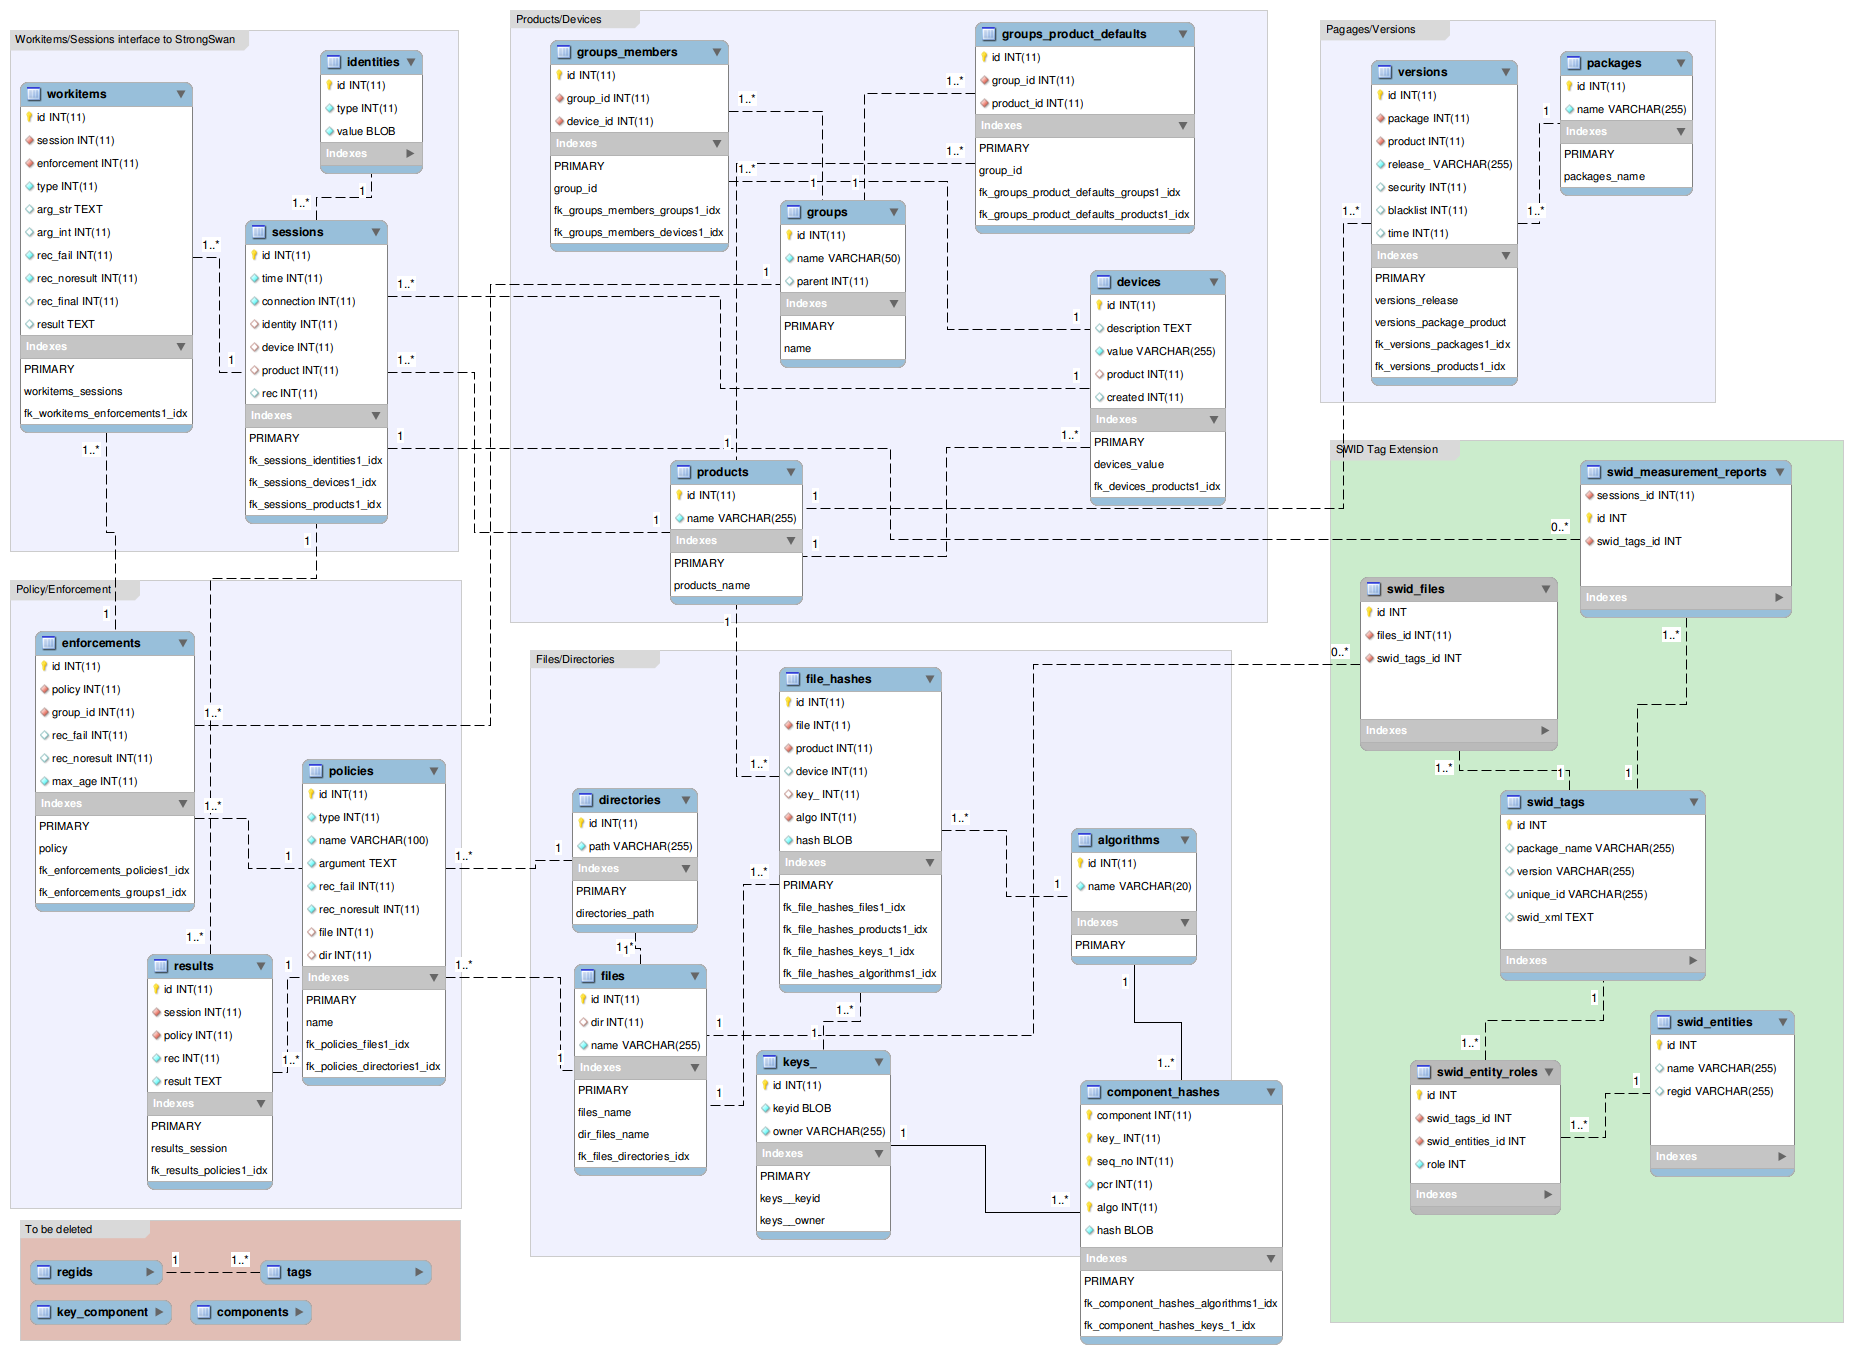
\includegraphics[width=0.7\linewidth]{./images/db/database-model}
\caption{}
\label{fig:database-model}
\end{figure}


\section{Verbesserungen}

\subsection{Multi-Rollen Konzept}

\subsubsection{Einleitung}

Um die Informationen in strongTNC zu Präsentationszwecken zugänglich machen zu können, 
ohne dass Änderungen vorgenommen werden können, weder absichtlich noch aus Versehen, 
soll eine Read-Only Rolle eingeführt werden.


\subsubsection{Ziel}

In einem ersten Schritt soll ein Rollen-Modell mit zwei Rollen eingeführt werden. 
Eine Rolle für Read-Only Zugriff und eine für den Vollzugriff. Der Zugriff soll, 
so wie es gegenwärtig implementiert ist, nicht personalisiert sein. Die Möglichkeit, 
den Login zu personalisieren sollte nicht grundsätzlich ausgeschlossen werden, jedoch 
steht die Implementation eines nicht personalisierten Read-Only Zugriffs im Vordergrund.


\subsubsection{Technische Umsetzung}

Django hat ein vollständiges Authentication- und Permission-System integriert. Damit 
lassen sich komplexe Permission-Szenarien abbilden, jedoch besteht auch die Möglichkeit 
nur Teile daraus zu verwenden und so ein einfacheres Rollen-Modell zu simulieren.

\paragraph*{User / Permissions}

Wenn keine personalisierten Login erwünscht sind, werden zwei technische User
erstellt, die für die beiden Rollen stehen. Das heisst es gibt beispielsweise
einen User \texttt{admin-user} und einen User \texttt{readonly-user}. Dem
\texttt{admin-user} wird die Permission \texttt{write\_access} erteilt, diese
Permission kann dann mittels \texttt{@permission\_required()} Decorator geprüft
werden.

Diese Umsetzungsvariante erlaubt es mit sehr wenig Aufwand personaliserte Logins
einzuführen. Für die Verwaltung der User stellt Django ein Admin-Interface zur
Verfügung, dieses müsste also nicht selber entwickelt werden.

\paragraph*{Templates}

In den Templates können die Permissions über das perms Objekt im Context geprüft werden. 
Beispiel:

\begin{pythoncode}

    <p>Read-write access.</p>

\end{pythoncode}

\paragraph*{Alternativen}

Als Alternative zum Permission-System könnten auch die standardmässig vorhandenen Flags 
\texttt{user.is\_admin} und \texttt{user.is\_staff} verwendet werden. Dies wäre bedeutend 
einfacher zu implementieren, die Lösung ist jedoch nicht ausbaufähig. Deshalb wird das 
Permission-System bevorzugt.


\subsubsection{Frontend Änderungen}
Folgende Änderungen müssen im User Interface vorgenommen werden.

\paragraph*{Login Screen}

Es muss eine Auswahl für die gewünschte Rolle zur Verfügung stehen. Diese kann bei zwei fix 
definierten Gruppen als Dropdown realisiert werden. Optional kann auch ein Inputfeld mit einem 
Username verwendet werden. 

\begin{figure}[H]
	\centering
	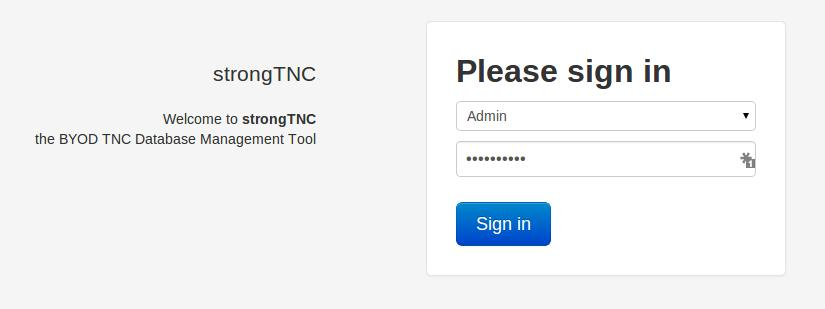
\includegraphics[width=\textwidth]{images/rollen-konzept/login-admin.jpg}
	\caption{Mögliches Aussehen der Loginmaske für den Adminlogin}
\end{figure}

\begin{figure}[H]
	\centering
	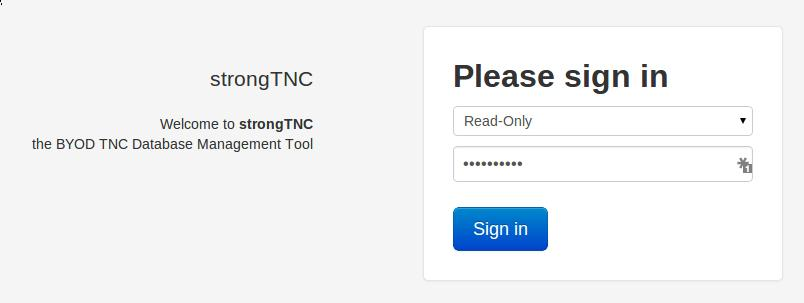
\includegraphics[width=\textwidth]{images/rollen-konzept/login-read-only.jpg}
	\caption{Mögliches Aussehen der Loginmaske für den Read-Only-Zugriff}
\end{figure}

\subsubsection{Configuration- und Data-Templates}

Alle Form-Elemente die einen Input erlauben werden deaktiviert, dies kann durch das 
Hinzufügen des HTML-Attribut \text2tt{disabled} erreicht werden. Alle Buttons werden entfernt.

\paragraph{Ausnahmen} \hspace{0pt} \\
\begin{itemize}
    \item In allen Views, das Filter-Feld
    \item In der Device-View, der Button "View device report"
\end{itemize}

\begin{figure}[H]
	\centering
	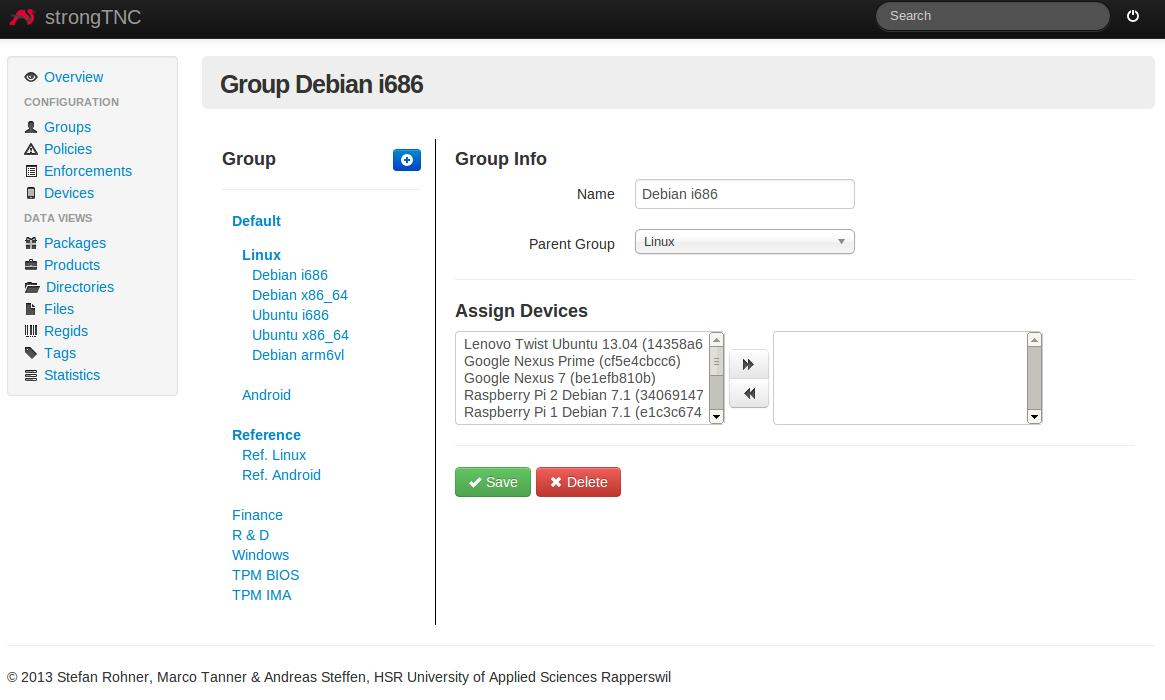
\includegraphics[width=\textwidth]{images/rollen-konzept/group-view-admin.jpg}
	\caption{Mögliches Aussehen der einer View für den Vollzugriff, am Beispiel der aktuellen Group-View}
\end{figure}

\begin{figure}[H]
	\centering
	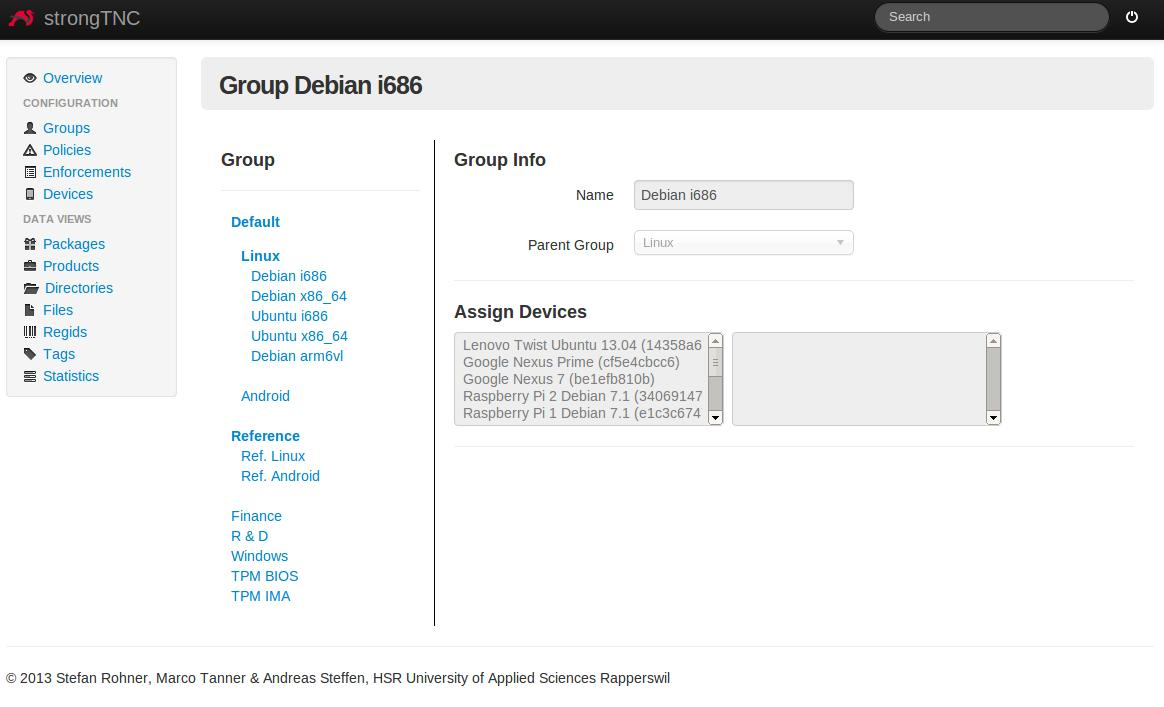
\includegraphics[width=\textwidth]{images/rollen-konzept/group-view-read-only.jpg}
	\caption{Mögliches Aussehen der einer View für den Read-Only Zugriff, am Beispiel der aktuellen Group-View}
\end{figure}


\subsubsection{Backend Änderungen}

Die meisten Views sind sehr ähnlich aufgebaut und verfügen über die gleichen Grundfunktionen, 
diese sind wie folgt einzuschränken:

\begin{description}
    \item [\texttt{models}] Nicht eingeschränkt
    \item [\texttt{model}] Nicht eingeschränkt
    \item [\texttt{add}] Eingeschränkt, nur für Admin
    \item [\texttt{save}] Eingeschränkt, nur für Admin
    \item [\texttt{delete}] Eingeschränkt, nur für Admin
    \item [\texttt{search}] Nicht eingeschränkt
    \item [\texttt{check}] Eingeschränkt, nur für Admin
\end{description}

Mit \texttt{models}, bzw. \texttt{models} sind die Funktionen einer View gemeint, die jeweils mit dem
Namen des Models benannt sind, zum Beispiel in der View \texttt{policy\_views.py}, die Funktionen
\texttt{policy()} und \texttt{policies()}.

\paragraph{Ausnahmen} \hspace{0pt} \\

\textbf{Device View:}
\begin{description}
    \item [\texttt{report} ] Nicht eingeschränkt
    \item [\texttt{session} ] Nicht eingeschränkt
\end{description}

\textbf{Package View:}
\begin{description}
    \item [\texttt{toggle\_version}] Eingeschränkt, nur für Admin
\end{description}



\section{Trennung, API Konzept}

